\chapter*{Update spyder dan Anaconda }

\begin{enumerate}
	\item Mengupdate melalui Anaconda Navigator, pertama klik Enviroments
	\begin{figure} [h]
	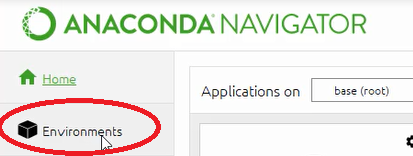
\includegraphics[width=5cm]{update/1.png}
	\centering
	\end{figure}
	
	\item Lalu search spyder dan pilih spyder 
	\begin{figure} [h]
	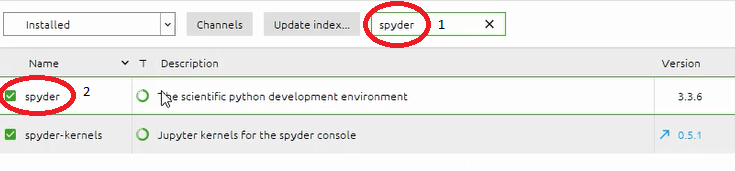
\includegraphics[width=5cm]{update/2.png}
	\centering
	\end{figure}

	\item Lalu ikuti seperti digambar dan pilih versi yang paling terbaru. Karena spyder saya telah paling ter update  
	\begin{figure} [h]
	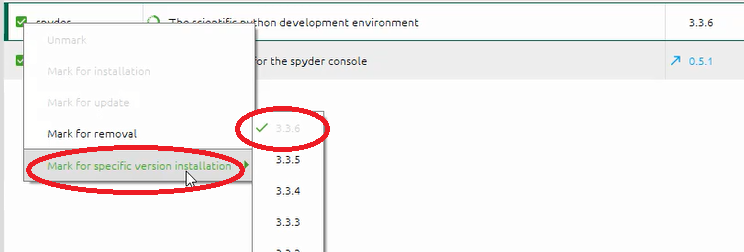
\includegraphics[width=5cm]{update/3.png}
	\centering
	\end{figure}
	
	\item mengupdate Anaconda sama hal nya seperti mengupdate spyder hanya berbeda saat mecari, ketikan "Anaconda" dan ikuti seperti digambar
	\begin{figure} [h]
	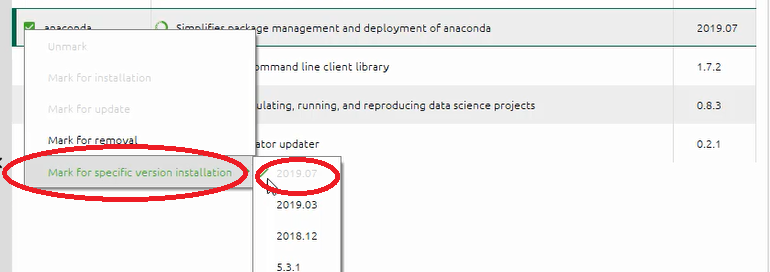
\includegraphics[width=5cm]{update/4.png}
	\centering
	\end{figure}
	

\end{enumerate}

